%%%%%%%%%%%%%%%%%%%%%%%%%%%%%%%%%%%%%%%%%
% Quick Start Example
%
% $Date$
% $Rev$:
% $Author$


\chapter{Quick Start Example}\label{chap:example}

This chapter provides a brief introduction to \Kieker{} based on a simple Bookstore example application. Section~\ref{sec:example:downloadInstall} explains how to download and install \Kieker{}. The Bookstore application itself is introduced in Section~\ref{sec:example:bookstore}, while the following sections demonstrate how to use \Kieker{} for monitoring~(Section~\ref{sec:example:monitoring}) and analyzing~(Section~\ref{sec:example:analysis}) the resulting monitoring data.

%%
\section{Download and Installation}\label{sec:example:downloadInstall}

The \Kieker{} download site\footnote{\KiekerDownloadURL{}} provides archives of the binary and source distribution, the Javadoc~API, as well as additional examples. For this quick start guide, \Kieker{}'s binary distribution, e.g., \file{\binaryFileForDownload}, is required and must be downloaded. After having extracted the archive, you'll find the directory structure and contents shown in Figure~\ref{fig:binary-layout}.

\enlargethispage{0.8cm}

% Note: The indention is not really necessary, but the tree is easier to understand in the tex-source.
\begin{figure}[h!]%[H]
\begin{graybox}
\dirtree{%
  .1 \DirInDirTree{\KiekerDir/}.
    .2 \DirInDirTree{bin/}\DTcomment{Call scripts for \Kieker{} tools}.
      .3 \ldots.
    .2 \DirInDirTree{dist/}\DTcomment{The \Kieker{} framework libraries}.
      .3 \mainJar.
      .3 \ldots. %\servletWar.
    .2 \DirInDirTree{doc/}\DTcomment{}.
      .3 kieker-\version\_userguide.pdf\DTcomment{PDF file of this document}.
    .2 \DirInDirTree{examples/}.
      .3 \DirInDirTree{userguide/}\DTcomment{Source code of the examples in this document}.
                        .4 \ldots.
    .2 \DirInDirTree{lib/}\DTcomment{Libraries required by \Kieker{}}.
%       .3 \commonsLoggingJar.
      .3 \ldots.
    .2 \DirInDirTree{META-INF/}\DTcomment{Example configuration files}.
      .3 \kiekerMonitoringProperties{}.
      .3 \ldots.
}
\end{graybox}
\caption{Directory structure and contents of \Kieker{}'s binary distribution}
\label{fig:binary-layout}
\end{figure}

\pagebreak

The Java sources presented in this user guide, as well as pre-compiled binaries, are included in the \file{\exampleDir/} directory. The file \file{\mainJar{}} contains the \KiekerMonitoringPart{} and \KiekerAnalysisPart{} components, as well as the \KiekerTraceAnalysis{} tool. The sample \KiekerMonitoringPart{}
configuration file %
\file{\kiekerMonitoringProperties{}} will be detailed in Chapter~\ref{chap:componentsMonitoring}. %
In addition to the \file{\mainJar{}} file, the \file{dist/} directory includes %
variants of this \file{.jar} files with integrated third-party libraries. Additional %
information on these \file{.jar} files and when to use them will follow later in this document. %

% Since \Kieker{} uses the Apache Commons library~\cite{CommonsLogging-WebSite} as a logging interface, the file \file{\commonsLoggingJar} is the only dependency to a third-party library which is needed to execute \Kieker{} in any case.

%%
\section{Bookstore Example Application}\label{sec:example:bookstore}

The Bookstore application is a small sample application resembling a simple bookstore with a market-place facility where users can search for books in an online catalog, and subsequently get offers from different book sellers.
Figure~\ref{fig:bookstore:classAndSequenceDiagrams} shows a class diagram describing the structure of the bookstore and a sequence diagram illustrating the dynamics of the application.

\begin{figure}[h]\centering
\subfigure[]{\label{fig:boostore:classdiagram}%
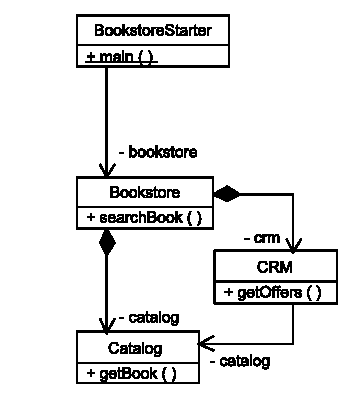
\includegraphics[scale=0.83]{images/kieker_bookstoreclassdiagram}%
}%
\subfigure[]{\label{fig:boostore:sequencediagram}%
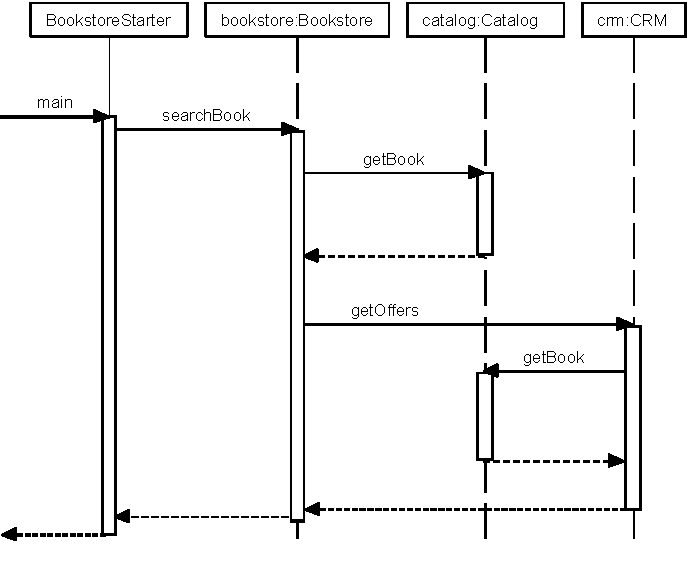
\includegraphics[scale=0.83]{images/kieker_SequenceDiagram-manually-changed}%
}
\caption{UML class diagram~\subref{fig:boostore:classdiagram} and sequence diagram~\subref{fig:boostore:sequencediagram} of the Bookstore application}
\label{fig:bookstore:classAndSequenceDiagrams}
\end{figure}

\pagebreak

The bookstore contains a catalog for books and a customer relationship management system~(CRM) for the book sellers. To provide this service, the different classes provide operations to initialize the application, search for books, and get offers or searched books. In this example, the methods implementing these operations are merely stubs. However, for the illustration of \Kieker{} they are sufficient and the inclined reader may extend the application into a real bookstore.

The directory structure of the Bookstore example is shown in Figure~\ref{fig:PlainBookstoreExample} and comprises four Java classes in its source directory \dir{src/.../ch2bookstore/} which are explained in detail below.

\begin{figure}[H]
\begin{graybox}
\dirtree{%
.1 \DirInDirTree{examples/}. %\DTcomment{The root directory of the project}.
.2 \DirInDirTree{userguide/}.
.3 \DirInDirTree{ch2--bookstore-application/}.
.4 \DirInDirTree{src/}\DTcomment{The directory for the source code files}.
.5 \DirInDirTree{.../ch2bookstore/}.
.6 Bookstore.java.
.6 BookstoreStarter.java.
.6 Catalog.java.
.6 CRM.java.
.5 build.properties.
.5 build.xml\DTcomment{Optional built script for the application}.
}
\end{graybox}

\caption{The directory structure of the Bookstore application}
\label{fig:PlainBookstoreExample}
\end{figure}

\NOTIFYBOX{The Java sources and a pre-compiled binary of the uninstrumented Bookstore application can be found in the \file{\plainBookstoreApplicationDirDistro{}/} directory.}

\quad\

\enlargethispage{1cm}

\noindent The class \class{BookstoreStarter} contains the application's \method{main} method (shown in Listing~\ref{lst:class:BookstoreStarter}), i.e., the program start routine. It initializes the \class{Bookstore} and issues five search requests by calling the \method{searchBook} method of the \object{bookstore} object.

\medskip

\setJavaCodeListing
\lstinputlisting[caption=\method{main} method from BookstoreStarter.java,firstline=23,firstnumber=23,lastline=29,label=lst:class:BookstoreStarter]{\plainBookstoreApplicationDir/src/kieker/examples/userguide/ch2bookstore/BookstoreStarter.java}

\pagebreak

\noindent The \class{Bookstore}, shown in Listing~\ref{lst:class:Bookstore}, contains a catalog and a CRM object, representing the catalog of the bookstore and a customer relationship management system which can provide offers for books out of the catalog. The business method of the bookstore is \method{searchBook()} which will first check the catalog for books and then check for offers.

In a real application these methods would pass objects to ensure the results of the catalog search will be available to the offer collecting method. However, for our example we omitted such code.

\lstinputlisting[caption=Bookstore.java,label=lst:class:Bookstore,firstline=19,firstnumber=19]{\plainBookstoreApplicationDir/src/kieker/examples/userguide/ch2bookstore/Bookstore.java}

\noindent The customer relationship management for this application is modeled in the \class{CRM} class shown in Listing~\ref{lst:class:CRM}. It provides only a business method to collect offers by using the catalog for some lookup. The additional catalog lookup is later used to illustrate different traces in the application.

\lstinputlisting[caption=CRM.java,label=lst:class:CRM,firstline=19,firstnumber=19]{\plainBookstoreApplicationDir/src/kieker/examples/userguide/ch2bookstore/CRM.java}

% \pagebreak

\enlargethispage{0.8cm}

\noindent Finally, the class \class{Catalog} is shown in Listing~\ref{lst:class:Catalog}. It resembles the catalog component in the application.

\lstinputlisting[caption=Catalog.java,label=lst:class:Catalog,firstline=19,firstnumber=19]{\plainBookstoreApplicationDir/src/kieker/examples/userguide/ch2bookstore/Catalog.java}

\noindent After this brief introduction of the application and its implementation, the next step is to see the example running. To compile and run the example, the commands in Listing~\ref{lst:bookstoreStarterNoInstr} can be executed. This document assumes that the reader enters the commands in the example directory. For this first example this is \dir{examples/userquide/ch2--bookstore-application/}.
\\
\NOTIFYBOX{Windows comes with two command-line interpreters called \texttt{cmd.exe} and \texttt{command.com}. Only the first one is able to handle wildcards correctly. So we recommend using \texttt{cmd.exe} for these examples.}

\setBashListing
% \begin{lstlisting}
nils@Laptop:~/example/$ javac src/mySimpleKiekerExampleManual/*.java -d build

nils@Laptop:~/example/$ java -classpath ./build/:./lib/commons-logging-1.1.1.jar\
                        mySimpleKiekerExampleManual.BookstoreMonitoringStarter 
\end{lstlisting}
% \WARNBOX{The default command-line interpreter of Windows doesn't support automatic file expansion. Therefore every single sourcefile has to be passed:
%\begin{lstlisting}[caption=Commands to compile and run the Bookstore application]
#\lstshellprompt{}# javac src/bookstoreApplication/Bookstore.java 
        src/bookstoreApplication/BookstoreStarter.java 
        src/bookstoreApplication/Catalog.java 
        src/bookstoreApplication/CRM.java 
        -d build/

#\lstshellprompt{}# java -classpath build/ bookstoreApplication.BookstoreStarter 
\end{lstlisting}
%
%}
\begin{lstlisting}[label=lst:bookstoreStarterNoInstr, caption=Commands to compile and run the Bookstore application]
> mkdir build
> javac src/kieker/examples/userguide/ch2bookstore/*.java -d build

> java -classpath build kieker.examples.userguide.ch2bookstore.BookstoreStarter
\end{lstlisting}

\noindent The first command compiles the application and places the resulting four class files in the \dir{build/} directory. To verify the build process, the \dir{build/} directory can be inspected. The second command loads the bookstore application and produces the output shown in Listing~\ref{lst:result-noinstr}.

\begin{lstlisting}[caption=Example run of the ``plain'' application,label=lst:result-noinstr]
Bookstore.main: Starting request 0
Bookstore.main: Starting request 1
Bookstore.main: Starting request 2
Bookstore.main: Starting request 3
Bookstore.main: Starting request 4
\end{lstlisting}


\noindent In this section, the \Kieker{} example application was introduced and when everything went well, the bookstore is a runnable program. Furthermore, the composition of the application and its function should now be present. %
The next Section~\ref{sec:example:monitoring} will demonstrate how %
to monitor this example application employing \KiekerMonitoringPart{} using manual instrumentation.

\pagebreak

%%
\section{Monitoring with \KiekerMonitoringPart{}}\label{sec:example:monitoring}

In the previous Sections~\ref{sec:example:downloadInstall} and \ref{sec:example:bookstore}, the \Kieker{} installation and the example application have been introduced. In this section, the preparations for application monitoring, the instrumentation of the application, and the actual monitoring are explained.

\quad\

\WARNBOX{In this example, the instrumentation is done manually. %
This means that the monitoring probe is implemented by mixing monitoring logic %
with business logic, which is often not desired since the resulting code is %
hardly maintainable. \Kieker{} includes probes %
based on AOP (aspect-oriented programming, \cite{Kiczales1997}) %
technology, as covered by Chapter~\ref{chap:aspectJ}. However, to illustrate the %
instrumentation in detail, the quick start example uses manual instrumentation.}

\

\noindent The first step is to copy the \Kieker{} jar-file \file{\mainJar} to the \dir{lib/} directory of the example directory~(see Section~\ref{sec:example:bookstore}). The file is located in the \dir{\KiekerDir/dist/} directory of the extracted \Kieker{} archive, as described in Section~\ref{sec:example:downloadInstall}. %
The final layout of the example directory is illustrated in Figure~\ref{fig:KiekerBookstoreExample}.

\begin{figure}[H]
\begin{graybox}
\dirtree{%
.1 \DirInDirTree{examples/}. %\DTcomment{The root directory of the project}.
.2 \DirInDirTree{userguide/}.
.3 \DirInDirTree{ch2--manual-instrumentation/}.
.4 \DirInDirTree{build/}\DTcomment{Directory for the Java class files}.
.4 \newFileDirInDirTree{\DirInDirTree{lib/}}\DTcomment{Directory for the required libraries}.
.5 \newFileDirInDirTree{\mainJar}.
.4 \DirInDirTree{src/}\DTcomment{The directory for the source code files}.
.5 \ldots.
}
\end{graybox}
\caption{The directory structure of the Bookstore application with \Kieker{} libraries}
\label{fig:KiekerBookstoreExample}
\end{figure}

\NOTIFYBOX{The Java sources and pre-compiled binaries of the manually instrumented Bookstore application described in %
this section can be found in the \file{\manualInstrumentedBookstoreApplicationDirDistro{}/} directory.}

\quad\

\noindent \Kieker{} maintains monitoring data as  so-called monitoring records. %
Section~\ref{sec:componentsMonitoring:monitoringRecords} describes how to define and use custom monitoring record types. %
The monitoring record type used in this example is an \textit{operation execution record} which %
is included in the \Kieker{} distribution. %
Figure~\ref{fig:OperationExecutionRecordClassDiagram} shows the %
attributes which  are relevant to this example. %
The record type will be detailed in Chapter~\ref{chap:aspectJ} .

\begin{figure}[H]
\begin{centering}
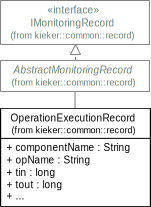
\includegraphics[scale=1]{images/kieker_OperationExecutionRecord-notraceattributes-inheritance}%
\caption{The class diagram of the operation execution record}
\label{fig:OperationExecutionRecordClassDiagram}
\end{centering}
\end{figure}

\noindent The attributes relevant to this part are \method{operationSignature} and \method{hostname}, %
as well as \method{tin} and \method{tout} for %
the timestamps before and after the call of the instrumented method.

\enlargethispage{1.2cm}

Listing~\ref{lst:cuttingBookstore} shows the instrumentation of the \class{Bookstore} class and its method \method{searchBook()}. In the lines~25 and~26, the monitoring controller is instantiated. It provides the monitoring service for the instrumentation.

% \TODO{Imports?!\\ --- avh: ja, evtl. mit linerange, aber er bl\"oderweise nummeriert er so durch}
% Make sure that this listing will be modified, once the sourcecode changes!!!
% It must show the whole monitoring of the bookstorecall, from getting the first time to persisting of the record!!

\setJavaCodeListing
\lstinputlisting[linerange={25-49}, firstnumber=25, caption=Instrumentation of the \method{getBook()} call in Bookstore.java, label=lst:cuttingBookstore]%
{\manualInstrumentedBookstoreApplicationDir/src/kieker/examples/userguide/ch2bookstore/manual/Bookstore.java}

\noindent The lines~32 and~34 are used to determine the current time in nanoseconds before and after the \method{getBook()} call. In lines~36 to~42, a monitoring record for this measurement is created and initialized, passing the method signature, the hostname, and the two time values as arguments. Finally the record is handed over to the monitoring controller (line~43) which calls a monitoring writer to persist the record. %
In this example, the filesystem writer is used---\Kieker{} uses this writer by default when no other writer is specified, %
as detailed in Section~\ref{sec:monitoring-log-writers}. %.

In addition to the instrumentation in the \class{Bookstore} class, the \method{getOffers()} method of the \class{CRM} class is instrumented as well. Similar to Listing~\ref{lst:cuttingBookstore}, measurements are taken before and after the call of the \object{catalog}'s \method{getBook()} method, as shown in %
lines~36 and~38 of Listing~\ref{lst:cuttingCRM}. Not shown in the listing is the instantiation of the monitoring controller. However, it is done in the same way as illustrated in Listing~\ref{lst:cuttingBookstore}. %And the complete example files can be found in the samples directory.
Finally, a record is created (see lines~40--46) and stored by calling the monitoring controller (see line~47).

\setJavaCodeListing
\lstinputlisting[firstline=34, firstnumber=34, lastline=48, caption=Instrumentation of the \method{getBook()} call in CRM.java, label=lst:cuttingCRM]%
{\manualInstrumentedBookstoreApplicationDir/src/kieker/examples/userguide/ch2bookstore/manual/CRM.java}

% \enlargethispage{0.5cm}

\noindent %
The next step after instrumenting the code is running the instrumented application. Listing~\ref{lst:bookstoreStarterLinux} shows the commands to compile and run the application under \UnixLikeSystems{}. Listing \ref{lst:bookstoreStarterWin} shows the same commands for Windows. The expected working directory is the base directory of this example, i.e. %
 \dir{\manualInstrumentedBookstoreApplicationDirDistro{}/}.
 
\pagebreak

% \enlargethispage{1cm}

\setBashListing
\begin{lstlisting}
nils@Laptop:~/example$ javac src/mySimpleKiekerExampleManual/*.java\
 -classpath ./lib/°\commonJar°:./lib/°\monitoringJar°:\
 -d build

nils@Laptop:~/example$ java\
-classpath ./build/:\
./lib/°\commonJar°:./lib/°\monitoringJar°:./lib/°\commonsLoggingJar°\
mySimpleKiekerExampleManual.BookstoreMonitoringStarter 
\end{lstlisting}


% \quad\

\WARNBOX{%
Under Windows it is necessary to separate the classpath elements by %
a semicolon instead of a colon. Also, we recommend to use the Windows shell %
\file{cmd.exe} for this tutorial since problems have been reported for the %
Windows PowerShell.}

% \pagebreak

\begin{lstlisting}[caption=Commands to compile and run the instrumented Bookstore under Windows,label=lst:bookstoreStarterWin]
#\lstshellprompt{}# mkdir build
#\lstshellprompt{}# javac src\bookstoreApplication\*.java -classpath lib\#\mainJar# -d build\

#\lstshellprompt{}# java -classpath build\;
       lib\#\mainJar#;
       lib\#\commonsLoggingJar#
       bookstoreApplication.BookstoreStarter 
\end{lstlisting}


\quad\

\noindent If everything worked correctly, a new directory for the monitoring data with a name similar to \dir{kieker-20120402-163314855-UTC-myHost-KIEKER-SINGLETON/} is created % in the default temporary directory
(see Figure~\ref{fig:logtree}). %
% The numbers in the directory name represent the time and date of the monitoring. %Thus, they will be different numbers for every run.
In \Kieker's default configuration, the log directory can be found in the default temporary directory: %
under \UnixLikeSystems{}, this is typically \dir{/tmp/}; %
check the environment variables \dir{\$TMPDIR} or \dir{\%temp\%} for the location under Mac OS or Windows respectively. %
The exact location of the created monitoring log is reported in \Kieker's console output (see for example Appendix~\ref{sec:appendix:manualInstrumentation:output}).
%it \dir{C:\textbackslash{}users\textbackslash{}[\ldots]\textbackslash{}temp} under Windows.
The monitoring directory contains two types of files: \dir{.dat} files containing text representations of the monitoring records and a %single
file named \dir{kieker.map} which contains information on the types of monitoring records used.

\begin{figure}[H]
\begin{graybox}
\dirtree{%
.1 \DirInDirTree{/tmp/}.
.2 \DirInDirTree{kieker-20120402-163314855-UTC-myHost-KIEKER-SINGLETON/}.
.3 kieker.map.
.3 kieker-20120402-163314882-UTC--000-Thread-1.dat.
}
\end{graybox}
\caption{Directory structure after a monitoring run}
\label{fig:logtree}
\end{figure}

\enlargethispage{1.5cm}

The Listings~\ref{lst:exampledat} and \ref{lst:examplemap} show example file contents. The \file{.dat}-file is saved in CSV format (\textbf{C}omma \textbf{S}eparated \textbf{V}alues)---in this case, the values of a monitoring record are separated by semicolons. To understand the \file{.dat}-file structure the semantics have to be explained. For this quick start example only some of the values are relevant. The first value \verb!$1! indicates the record type. The fourth value indicates the class and method which has been called. And the seventh and eighth value are the start and end time of the execution of the called method.

\setBashListing
\lstinputlisting[caption=kieker-20120402-163314882-UTC--000-Thread-1.dat (excerpt), firstline=1, lastline=2, label=lst:exampledat]%
{ch2-quickstart-example/kieker-20120402-163314855-UTC-myHost-KIEKER-SINGLETON/kieker-20120402-163314882-UTC--000-Thread-1.dat}

\noindent The second file is a simple mapping file referencing keys to monitoring record types. In Listing~\ref{lst:examplemap} the key \verb!$1! is mapped to the type of operation execution records which were used in the monitoring. The key value corresponds to the key values in the \file{.dat}-file.

\lstinputlisting[caption=kieker.map, label=lst:examplemap]%
{ch2-quickstart-example/kieker-20120402-163314855-UTC-myHost-KIEKER-SINGLETON/kieker.map}

\noindent By the end of this section, two Java classes of the Bookstore application %
have been manually instrumented using \KiekerMonitoringPart{} and at least one %
run of the instrumented application has been performed. %
The resulting monitoring log, written to the \file{.dat}-file in CSV format, could %
already be used for analysis or visualization by any spreadsheet or %
statistical tool. %
The following Section~\ref{sec:example:analysis} will show how to process %
this monitoring data with \KiekerAnalysisPart{}.

%%
\section{Analysis with \KiekerAnalysisPart{}}\label{sec:example:analysis}

%The last task of a successful application monitoring is the analysis of the collected information.
In this section, the monitoring data recorded in the previous section is %
analyzed with \KiekerAnalysisPart{}. %
% The second step is to write a suitable analyzer. And finally the analyzer is used to aggregate the information in a sensible way.
For this quick example guide, the analysis tool is very simple and does not show %
the full potential of \Kieker{}. For more detail, read %
Chapter~\ref{chap:componentsAnalysis} to learn which plugins, i.e., readers %
and filters, are included in \Kieker{}, how to use them, and how to develop %
custom plugins. %
Chapter~\ref{chap:aspectJ} presents the \KiekerTraceAnalysis{} tool, which %
is also based on \KiekerAnalysisPart{}.
\KiekerAnalysisPart{} has a dependency to the Eclipse Modeling Framework~(EMF).%
\footnote{\url{http://www.eclipse.org/modeling/emf/}} %
For this reason, we are using the \file{\mainJarEMF{}} that is a variant of %
the \file{\mainJar{}}, additionally including the required EMF dependencies. %
When using the \file{\mainJar{}}, the \file{org.eclipse.emf.\-*.jar} files (to %
be found in \Kieker's \file{lib/} directory) need to be added to the classpath. %

\begin{figure}[H]
\begin{graybox}
\dirtree{%
.1 \DirInDirTree{examples/}. %\DTcomment{The root directory of the project}.
.2 \DirInDirTree{userguide/}.
.3 \DirInDirTree{ch2--manual-instrumentation/}.
.4 \DirInDirTree{build/}\DTcomment{Directory for the Java class files}.
.4 \newFileDirInDirTree{\DirInDirTree{lib/}}\DTcomment{Directory for the required libraries}.
.5 \newFileDirInDirTree{\mainJarEMF}.
.4 \DirInDirTree{src/}\DTcomment{The directory for the source code files}.
.5 \DirInDirTree{.../manual/}.
.6 \ldots.
.6 \newFileDirInDirTree{BookstoreAnalysisStarter.java}.
}
\end{graybox}
\caption{Directory layout of the example application with the analysis files highlighted}
\label{lst:analysisExampleLayout}
\end{figure}

\noindent The analysis application developed in this section comprises the file %
\file{BookstoreAnalysisStarter.java}, as shown in Figure~\ref{lst:analysisExampleLayout}. %
This file can also be found in the directory \dir{\manualInstrumentedBookstoreApplicationDirDistro{}/}.
The file sets up the basic pipe-and-filter configuration depicted in Figure~\ref{fig:example:ch2:pipe-and-filter}: %
\Kieker{}'s file system reader (\class{FSReader}) reads monitoring records %
from a file system monitoring log (as produced in the previous Section~\ref{sec:example:monitoring}) %
and passes these to the \class{TeeFilter} plugin; the \class{TeeFilter} plugin %
reads events of arbitrary type (i.e., Java \class{Object}), prints them to a %
configured output stream, and also relays them to filters connected to the %
filter's output port \method{relayedEvents}. %

\begin{figure}[h]
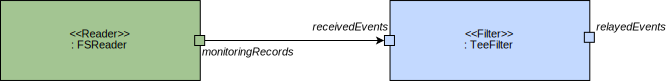
\includegraphics[width=\textwidth]{images/ch2-example-pnp}
\caption{Example pipe-and-filter configuration}
\label{fig:example:ch2:pipe-and-filter}
\end{figure}

Currently, \KiekerAnalysisPart{} pipe-and-filter configurations can only %
be created programmatically, i.e., by configuring, instantiating, and %
connecting the plugins in a Java program. %
For the example, this is demonstrated in Listing~\ref{lst:BookstoreAnalysisStarter}, %
which shows an excerpt from the \class{BookstoreAnalysisStarter}'s \method{main} %
method. %

\pagebreak

\setJavaCodeListing
\lstinputlisting[gobble=4,caption=BookstoreAnalysisStarter.java (excerpt from \method{main} method),label=lst:BookstoreAnalysisStarter,firstline=37,firstnumber=36,lastline=56]%
{\manualInstrumentedBookstoreApplicationDir/src/kieker/examples/userguide/ch2bookstore/manual/BookstoreAnalysisStarter.java}

% \pagebreak

\noindent The \class{BookstoreAnalysisStarter} follows a simple scheme. Each %
analysis tool has to create at least one \class{AnalysisController} which can be %
seen in Listing~\ref{lst:BookstoreAnalysisStarter} in line~37. Then, the plugins, %
which may be readers or filters, are configured, and instantiated. The usage of the  %
constructor ensures that the component is registered with the analysis instance. %
Lines~40--42 configure, instantiate, and register the file system monitoring %
log reader, which uses the command-line argument value as the input directory. %
The application expects the %
output directory from the earlier monitoring run (see Section~\ref{sec:example:monitoring}) %
as the only argument value, which must be passed manually. %
Lines~45--48 configure, instantiate, and register the \class{TeeFilter}, %
which outputs received events to the standard output. Lines~51 and~52 connect %
the \class{TeeFilter}'s input port to the filesystem reader's output port. %
The analysis is started by calling its \method{run} method (line~54). %


The Listings~\ref{lst:bookstoreAnalysisStarterLinux} and \ref{lst:bookstoreAnalysisStarterWin} %
describe how the analysis application can be compiled and executed under \UnixLikeSystems{} and Windows.

\setBashListing
\enlargethispage{1.0cm}
\begin{lstlisting}[caption=Commands to compile and run the analysis under \UnixLikeSystems{},label=lst:bookstoreAnalysisStarterLinux] 			
#\lstshellprompt{}# mkdir build
#\lstshellprompt{}# javac src/kieker/examples/userguide/ch2bookstore/manual/*.java 
        -classpath lib/#\mainJarEMF# -d build/

#\lstshellprompt{}# java -classpath build/:lib/#\mainJarEMF#
       kieker.examples.userguide.ch2bookstore.manual.BookstoreAnalysisStarter 
       /tmp/kieker-20120402-163314855-UTC-myHost-KIEKER-SINGLETON
\end{lstlisting}	

\begin{lstlisting}[caption=Commands to compile and run the analysis under Windows,label=lst:bookstoreAnalysisStarterWin]
#\lstshellprompt{}# mkdir build
#\lstshellprompt{}# javac src\kieker\examples\userguide\ch2bookstore\manual\*.java 
        -classpath lib\#\mainJarEMF# -d build\

#\lstshellprompt{}# java -classpath build\;lib\#\mainJarEMF#
       kieker.examples.userguide.ch2bookstore.manual.BookstoreAnalysisStarter 
       C:\Temp\kieker-20130910-120352847-UTC-myHost-KIEKER-SINGLETON
\end{lstlisting}	



\noindent You need to make sure that the application gets the correct path from the monitoring run.
The \class{TeeFilter} prints an output message for each record received. %
An example output can be found in Appendix~\ref{sec:appendix:manualInstrumentation:output}.
% A possible display of the run can be found in the appendix of this tutorial.
